% latex-beamer, texlive-publishers, texlive-latex-extra
%
%
\documentclass{beamer}
\usetheme{Luebeck}
\usecolortheme{default}
\usefonttheme{professionalfonts}
\usefonttheme[onlymath]{serif}
%\usefonttheme[onlylarge]{structurebold}
%\setbeamerfont{title}{family=\rm}
%\setbeamerfont*{frametitle}{size=\normalsize,series=\bfseries}
%\setbeamertemplate{navigation symbols}{}

\begin{document}

\title[\textbf{DAE Tools} - Introduction]{\textbf{DAE Tools}: An equation-oriented process\linebreak modelling and optimization software}
\subtitle{\textbf{Introduction}}
\author{Dragan Nikolic}
\institute
{
  University of Western Macedonia\\
  Department of Mechanical Engineering\\
  50100 Kozani, Greece
}
%\logo{\includegraphics{../images/[d][a][e]_Tools_project.png}}
\date{\today} 
\titlegraphic{\includegraphics{../[d][a][e]_Tools_project.png}}

\AtBeginSection[]
{
  \begin{frame}
    \frametitle{Outline}
    \tableofcontents[currentsection]
  \end{frame}
}

\begin{frame}
\titlepage
\end{frame}

\begin{frame}
\frametitle{Outline}
\tableofcontents[currentsubsection, 
                 hideothersubsections, 
                 sectionstyle=show, 
                 subsectionstyle=hide]
\end{frame} 


\section{Intro}

\subsection{General Info}
\begin{frame}
\frametitle{What is DAE Tools?} 
\begin{itemize}
  \item Process modelling, simulation, optimization and parameter estimation software (www.daetools.com)
  \item Areas of application:
    \begin{itemize}
      \item Initially: chemical process industry (mass, heat and momentum transfers, chemical reactions, separation processes, phase-equilibrium, thermodynamics)
      \item Nowadays: multi-domain
    \end{itemize}
  \item Hybrid approach between general-purpose programming languages (c++, Fortran, Java) and domain-specific modelling languages (Modelica, gPROMS...)
\end{itemize}
\end{frame}

\begin{frame}
\frametitle{What can be done with DAE Tools?} 
\begin{itemize}
  \item Simulation
    \begin{itemize}
      \item Steady-State 
      \item Transient
    \end{itemize}
  \item Optimization
    \begin{itemize}
      \item NLP problems: IPOPT, NLOPT, OpenOpt, scipy.optimize
      \item MINLP problems: BONMIN
    \end{itemize}
  \item Parameter estimation: Levenberg–Marquardt algorithm (scipy.optimize)
\end{itemize}
\end{frame}

\begin{frame}
\frametitle{Types of systems that can be modelled}
\begin{itemize}
  \item Initial value problems of implicit form: systems of linear, non-linear, and (partial-)differential algebraic equations
  \item Index-1 DAE systems
  \item With lumped or distributed parameters: Finite Difference or Finite Elements Methods
  \item Steady-state or dynamic
  \item Continuous with some elements of event-driven systems (discontinuous equations, state transition networks and discrete events) 
\end{itemize}
\end{frame}

\subsection{Motivation}
\begin{frame}
\frametitle{Why yet another software?}
Advantages:
\begin{enumerate}
  \item Hybrid approach betwen DSL and GPPL
  \item Programmatical generation of models
  \item Runtime modification of objcts/models (operating procedures)
  \item Introperability with 3rd party software packages/libraries
  \item Code generation/Model exchange capabilities
\end{enumerate}
\end{frame}

\subsection{Main features}
\begin{frame}
\frametitle{Not a modelling language}
\begin{itemize}
  \item A set of software packages
  \item API for:
  \begin{itemize}
    \item Model development
    \item Results processing (plotting, various file formats)
    \item Simulation, optimization and parameter estimation
    \item Code generation for other DSLs and programming languages
    \item Report generation (XML+MathML) and model exchange
  \end{itemize}
  \item Large set of supported solvers (DAE, LA, NLP, MINLP)
\end{itemize}
\end{frame}

\begin{frame}
\frametitle{Not a modelling language (cont'd)}
\begin{itemize}
  \item Allows easy interaction with other software libraries (two-way interoperability with other software, embedding in other software etc.)
  \item Free/Open source software (GNU GPL)
  \item Cross-platform (GNU/Linux, MacOS, Windows)
  \item Supports multiple architectures (32/64 bit x86, arm, any other with the GNU toolchain)
  \item Developed in c++ with Python bindings (Boost.Python)
\end{itemize}
\end{frame}

\begin{frame}
\frametitle{Object-oriented modelling}
\begin{itemize}
  \item Everything is an object
  \item Models are classes derived from the base daeModel class
  \item Basically all OO concepts supported by the target language (c++, Python) allowed, except few exceptions
  \item Multiple inheritance is supported
  \item Models can be parametrized (using templates in c++)
  \item Derived classes always inherit all declared parameters, variables, equations etc. (polymorphism achieved through virtual functions where the declaration takes place)
  \item All parameters, variables, equations etc. remain public
  \item Hierarchical model decomposition
\end{itemize}
\end{frame}

\begin{frame}
\frametitle{Equation-oriented (acausal) modelling}
\begin{itemize}
  \item Equations given in an implicit form (as a residual)
  \item Input-Output causality is not fixed
  \item Benefits:
  \item Increased model re-use
  \item Support for different simulation scenarios (based on a single model) by specifying different degrees of freedom
  \item For instance, equation given in the following form:

  \item can be used to determine either x1, x2 or x3 depending on what combination of variables is known:
\end{itemize}
\end{frame}

\begin{frame}
\frametitle{Separation of models definition from operations on them}
\begin{itemize}
  \item The structure of the model (parameters, variables, equations etc.) is given in the model class while the runtime information in the simulation class 
  \item Single model definition, but:
  \item One or more different simulation scenarios
  \item One or more optimization scenarios
  \item Hybrid continuous/discrete systems 
  \item Continuous with some elements of event-driven systems (discontinuous equations, state transition networks and discrete events)
\end{itemize}
\end{frame}

\begin{frame}
\frametitle{Code generation}
\begin{itemize}
  \item Model export from DAE Tools to other DSL or programming languages)
  \item Modelica
  \item ANSI C
  \item Support for Functional Mock-up Interface for Model Exchange and Co-Simulation (FMI): https://www.fmi-standard.org 
  \item FMI – a tool independent standard to support both model exchange and co-simulation of dynamic models using a combination of xml-files and compiled C-code
  \item Still in experimental phase
\end{itemize}
\end{frame}

\begin{frame}
\frametitle{Model reports}
\begin{itemize}
  \item Automatic model documentation
  \item XML + MathML format
  \item Two types:
  \item Model description report (contains model definition)
  \item Runtime report with all values and equations expanded (contains definition of the simulation)
  \item XSL transformation used to to generate HTML code and visualize reports 
\end{itemize}
\end{frame}



\section{Programming paradigms}
\subsection{Approaches to process modelling}
\begin{frame}\frametitle{unnumbered lists}
\end{frame}

\begin{frame}\frametitle{lists with pause}
\end{frame}

\subsection{Comparison of DSL and DAE Tools Approach}
\begin{frame}\frametitle{numbered lists}
\end{frame}

\begin{frame}\frametitle{numbered lists with pause}
\end{frame}

\section{Use Cases} 
\subsection{NineML}
\begin{frame}\frametitle{Tables}
\end{frame}

\end{document}